%%%%%%%%%%%%%%%%%%%%%%%%%%%%%%%%%%%%%%%%%%%%%%%%%%%%%%%%%%%%%%%%%%%%%%%%
%
% M2修論テンプレート For UTF-8
% created by: kohei-y at Dec. 22, 2015
% modified by; kohei-y at Jan. 4, 2016
% modified by: kohei-y at Jan. 11, 2016(Thanks to yuki)
%
%%%%%%%%%%%%%%%%%%%%%%%%%%%%%%%%%%%%%%%%%%%%%%%%%%%%%%%%%%%%%%%%%%%%%%%%
\documentclass[12pt,a4paper,titlepage,report]{jsbook}
\usepackage{otf}
\usepackage{ascmac}
\usepackage{moreverb}

\usepackage[dvipdfmx]{graphicx}
\usepackage[dvipdfmx]{color}

\usepackage{listings, color}
\usepackage{booktabs}
\usepackage{multirow}

\definecolor{OliveGreen}{rgb}{0.0,0.6,0.0}
\definecolor{Orenge}{rgb}{0.89,0.55,0}
\definecolor{SkyBlue}{rgb}{0.28, 0.28, 0.95}
\lstset{
  basicstyle={\ttfamily},
  identifierstyle={\small},
  commentstyle={\smallitshape},
  keywordstyle={\small\bfseries},
  ndkeywordstyle={\small},
  stringstyle={\small\ttfamily},
	tabsize=2,
  frame={tb},
  breaklines=true,
  columns=[l]{fullflexible},
  numbers=left,
  xrightmargin=0zw,
  xleftmargin=2zw,
  numberstyle={\scriptsize},
  stepnumber=1,
  numbersep=1zw,
  lineskip=-0.5ex,
  keywordstyle={\color{SkyBlue}},     %キーワード(int, ifなど)の書体指定
  commentstyle={\color{OliveGreen}},  %注釈の書体
  stringstyle=\color{Orenge}          %文字列
}



\usepackage{afterpage,array,rotating}
\newcolumntype{Y}{>{\centering\arraybackslash}p{5em}}

\usepackage[hang,small,bf]{caption}
\usepackage[subrefformat=parens]{subcaption}
\captionsetup{compatibility=false}

% フォントが気に入らなかったら消して
\usepackage{newtxtext} % T1, lining figures so math uses lf
\usepackage[varqu]{zi4}% inconsolata
\usepackage{textcomp} % required for special glyphs

% これは数学系のおまじない.
\usepackage{amsmath}

% フォントが気に入らなかったら消して
\usepackage[varg,vvarbb,cmintegrals,cmbraces]{newtxmath}
\usepackage{bm} % load after all math to give access to bold math



% hyperref: ハイパーリンクをつける
\usepackage[dvipdfmx,CJKbookmarks=true,colorlinks,%おまじない
  allcolors=black,urlcolor=blue,citecolor=blue,%色の設定
  setpagesize=false,%ページサイズを変更しないように
  pdftitle={},%
  pdfauthor={},%
  pdfkeywords={keywords}%
]{hyperref}
\usepackage[dvipdfmx]{pxjahyper} % hyperrefを使った時のタイトルをUnicodeに




%%%%%%%%%%%%%%%%%%%%%%%%%%%%%%%%%%%%%%%%%%%%%%%%%%%%%%%%%%%%%%%%%%%%%%%%
%
%文書情報
%
\title{% 行数が多少増えても大丈夫な仕様
\vspace*{-6.0em}\sffamily\huge {\Huge 卒~業~論~文}\\[2.0em]{\vbox to9em{%
IoT機器を想定した実行環境における\\マルウェアの影響評価}}} % タイトル
\author{\LARGE\sffamily101910020~~~~~~大羽~~俊輔}% 名前
\date{%
% ↓が所属,↓↓が日付(日付以外は書き換えることないと思うけど……)
\LARGE\vspace{1.0em}\sffamily 名古屋大学~~情報学部\\コンピュータ科学科~~情報システム系\\%
2023年2月}% 日付
%%%%%%%%%%%%%%%%%%%%%%%%%%%%%%%%%%%%%%%%%%%%%%%%%%%%%%%%%%%%%%%%%%%%%%%%




\begin{document}

\newpage
\maketitle
%%
\chapter*{{\normalsize 概要}\vspace*{-3\Cvs}}
\addcontentsline{toc}{chapter}{概要}
IoT機器の増加に伴い、マルウェアによるIoT機器への攻撃リスクが高まっている。IoTとは、実世界のモノをインターネットに接続し、インターネットを介して情報を相互にやり取りするという考え方である。マルウェアはコンピュータの普及に伴い盛んに研究されてきた分野であるが、IoT機器を攻撃対象としたマルウェアが盛んに研究されるようになったのは、IoT機器が普及してきた2018年頃のことである。パーソナルコンピュータの多くがx86\_64プロセッサで動作している一方で、IoT機器の多くはARMプロセッサで動作している。従来のマルウェアの解析・検出手法の多くはx86\_64アーキテクチャに特化しており、命令セットが異なるARMアーキテクチャに対して容易に転用できない。そのため、ARMアーキテクチャを攻撃対象としたマルウェアの更なる研究が求められている。昨今、IoT機器の実行環境としてコンテナやユニカーネルなどの環境が提案されており、実行環境は多様化してきている。特に、コンテナは近年注目されている環境である。

本研究では、IoT機器の実環境を想定した環境においてマルウェアがどのような影響を与えるのかを定量的に示すことを目的として、評価手法の提案とその手法を用いた評価実験を行う。アプリケーション実行環境として、ラズビアン環境、コンテナ環境、ユニカーネル環境を対象に、それぞれの環境においてマルウェアを実行した際に実行環境やサービスにどのような影響を与えるのかを評価する。いずれの環境も、IoT機器の機能としてウェブサーバを想定し、ウェブサーバアプリケーションをインストールする。評価指標として、マルウェアの実行可否および脅威スコアを用い、マルウェアの影響を定量的に推定する。実行の可否は、マルウェアが実行可能かどうかを示す指標であり、マルウェアを実行した結果が正常終了または一定時間実行状態であったものを実行可能、異常終了したものを実行不可と判定する。脅威スコアは、実行したマルウェアがどの程度脅威となるかを示す値であり、マルウェアの実行の可否とそのマルウェアの分類に応じて算出される。これらの指標を用いて各環境におけるマルウェアの影響を比較することで、3つの環境の特性を示すことができる。ラズビアン環境の評価環境として、エミュレータ型仮想化ソフトウェアであるQEMUを用いてRaspberry Pi OSを動作させ、マルウェアの実行、実行結果の取得、脅威スコア算出を自動化する環境を構築した。

評価実験の結果、実行の可否および脅威スコアを求めることに成功し、提案手法を用いることでマルウェアの影響を定量的に示すことが出来ることが分かった。加えて、実行に失敗したマルウェアの終了ステータスを分析することで、実行に失敗するマルウェアの多くが不正なメモリ参照または存在しないコマンドの参照により実行に失敗していることが明らかになり、使用可能なコマンドを制限することでマルウェアの影響を抑制できることを示唆する結果となった。自動化を行うことで、1つのマルウェアにつき180秒程度掛かっていた評価を100秒程度で行うことができ、提案手法の有用性が示された。

本研究では、IoT機器の実環境を想定した3つの実行環境においてマルウェアがどのような影響を与えるのかを定量的に示す手法を提案し、ラズビアン環境において実際に評価実験を行うことでその有効性を示した。今後の課題として、残る2つの環境でも評価実験を行うことや、脅威スコアを厳密に算出するために実際のマルウェアの振る舞いから脅威の程度を評価すること、評価にかかる時間をさらに短縮することなどが挙げられる。

%%


\pagenumbering{roman}
\tableofcontents
%% 図目次・表目次(お好みに合わせて)
\listoffigures
\listoftables
%%%%%%%%%%
\newpage


\pagestyle{plain}
\pagenumbering{arabic}


% ============= はじめに =============


\chapter{はじめに}
\section{研究背景}
\subsection{昨今のマルウェア情勢}
近年、マルウェアによる被害が増加している。特に、攻撃対象のシステムを暗号化し、復号と引き換えに金銭の支払いを求めてくるランサムウェアと呼ばれるマルウェアの活動が活発化している。ランサムウェアに感染すると、事業停止に陥ったり、機密情報が流出するなどの被害を被る可能性がある。警視庁の公開する「令和4年上半期におけるサイバー空間をめぐる脅威の情勢等について」\cite{policereport}によると、国内におけるランサムウェアによる被害の報告件数は2020年から年々増加しており、2022年には2020年のおよそ5倍の114件の被害が報告されている。また、情報処理推進機構(IPA)が公開している「情報セキュリティ10大脅威2022」\cite{bestthreat2022}では、組織部門において2021年に引き続きランサムウェアが脅威の1位として位置付けられており、現在のサイバー空間における大きな脅威となっている。

IoT機器においてもマルウェアの被害は報告されている。IoTとは、実世界のモノをインターネットに接続し、インターネットを介して情報を相互にやり取りするという概念である。IoT機器におけるマルウェアによる被害の多くは、ボット型マルウェアによるものであり、感染するとDDoS攻撃の踏み台に利用されるなどの被害が生じる。特に、2016年頃に大規模なDDoS攻撃を行ったことで知られるボットMiraiは、そのソースコードが公開されて以降、その亜種が出現し続けておりIoT機器にとって大きな脅威となっている\cite{malwaresurvey}。IoT機器がマルウェアに感染する原因の多くが、初期パスワードを変更していなかったりシステムの更新を行なっていないためだと言われている。情報通信研究機構(NICT)では、感染リスクのある機器を調査し利用者への注意喚起を行う取組、NOTICE\cite{notice}を通じてマルウェアに対する対策を講じている。

% IoT 機器増加の傾向についても触れる?この取り組みで改善されたが、今後も IoT 機器が増加していくことから引き続きマルウェアへの対策が必要である。

\subsection{マルウェア研究における研究対象の偏り}
現在、既存のマルウェアに関する研究の多くが、Windowsを研究対象としており、Linuxといったその他のOSを研究対象にしている研究は比較的少ない\cite{malwaresurvey}。Windowsを研究対象とする研究が多い背景としては、Windowsは他のOSに比べて利用ユーザが多く、それを狙うマルウェアが多く存在することから、積極的に研究が行われているためであると考えられる。近年、IoT機器を狙ったマルウェアの脅威の拡大に伴い、LinuxなどのOSを研究対象とする研究も報告されてきているが、Windowsを対象とする研究に比べて十分な議論はなされていない。

既存のマルウェアに関する研究の中で、ARMアーキテクチャ上で動作するマルウェアを研究対象とした研究は少ない。パーソナルコンピュータでは一般的にx86\_64プロセッサが用いられるのに対し、IoT機器などの多くの組み込み機器ではARMプロセッサが用いられることが一般的である\cite{malwaresurvey}。IoT機器が普及する以前、マルウェアの多くはパーソナルコンピュータを攻撃対象としていたためx86\_64アーキテクチャを対象とした研究が盛んに行われたが、ARMアーキテクチャを対象とした研究が行われるようになったのはIoT機器を狙うマルウェアが流行してきた比較的最近のことである\cite{malwaresurvey}。

マルウェアの研究において、アーキテクチャは重要な要素である。一般的にマルウェアの検出手法は特定のアーキテクチャに特化して提案されているため、既存の検出手法を異なるアーキテクチャに転用することは困難とされる。例えば、x86\_64アーキテクチャを対象にしたマルウェアの研究で提案された検出手法は、ARMアーキテクチャを対象にしたマルウェアの検出には転用できない。こうした背景から、ARMアーキテクチャを対象としたマルウェアの研究が急務となっている。

\section{研究目的と概要}
本研究は、ARMプロセッサのIoT機器を想定した3つの実行環境において、マルウェアが与える影響を定量的に評価し、環境ごとの影響を比較することを目的とする。
はじめに、影響評価を行う上での評価対象と評価指標を定め、評価実験のための環境構築を行なった。続いて、評価対象のうちラズビアン環境を用いて定量的なマルウェアの影響評価を行った。

% ARMとIoT機器は切り離すべきか?

本研究の貢献は、以下の通りである。
\begin{itemize}
    \item ARMプロセッサのIoT機器を想定した実行環境においてマルウェアが与える影響を定量的に示す手法を提案した
    \item 提案手法を用いた評価実験を行い、その有効性を示した
\end{itemize}

\section{本論文の構成}
本論文は、本章を含めて全5章で構成されている。2章では、関連研究としてIoTマルウェアの検出・分類手法とV-Sandboxについて述べる。3章では、評価を行う上での評価対象と評価指標を提案し、最後に環境構築について述べる。4章では、実験概要、実験結果、考察について述べる。5章では、本研究の結論とまとめ、今後の課題について述べる。


% ============= 関連研究 =============


\chapter{関連研究}
\section{IoTマルウェアの検出・分類手法}
IoT機器を攻撃対象としたマルウェアの検出・分類手法については、既に多くの議論が行われている。以降、IoT機器を攻撃対象としたマルウェアをIoTマルウェアと呼ぶこととする。IoTマルウェアに限らず、一般にマルウェアの解析には静的解析と動的解析の二つのアプローチが存在する\cite{malwaresurvey}。静的解析は、マルウェアのバイナリファイルから得られる構造的、意味的情報をプログラムを実行することなく分析する手法である。この手法では、アンチアセンブル、コード難読化などの解析回避手法の影響を受けやすいとされている。一方、動的解析は、マルウェアのプログラムを実行し、その挙動を観察したりデバッグを行うことで分析を行う手法である。この手法ではアンチデバッグや遅延実行の影響を受けやすいとされている。マルウェアを実行する際は一般的に、隔離された実行環境であるサンドボックス上で実行し、その挙動を分析する。本研究においても、サンドボックスを構築し動的解析による解析を行った。

IoTマルウェアの検出・分類手法として従来から機械学習が活用されており、学習のための様々な特徴量\cite{malwaresurvey}が提案されている。その中から、三つの特徴量について取り上げる。

\subsection{オペコード}
マルウェアの検出・分類を行う上で有効な特徴量として、オペコードが挙げられる。オペコードとはプロセッサが実行可能な命令のことであり、レジスタやオペランドを引数に取り、目的の動作を実行する。オペコードはマルウェアの検出・分類に有効なことがHamedらによって示されている\cite{opcode}。しかしながら、オペコードは命令セット・アーキテクチャに依存しているため、比較的汎用性に欠ける特徴量であると思われる。

\subsection{文字列データ}
プログラムのバイナリデータの中には、文字列として印字可能な文字列が含まれている場合があり、特徴量として用いることが可能である。例えば、IPアドレスやDLL名、エラーメッセージやコメントなどである。

\subsection{バイト列}
バイト列はバイナリデータをバイト単位で逐次的に表現した数値列である。NguyenらによってLinuxにおいて、いくつかのモデルが検出・分類に有効であることが示されている\cite{bytelinux}。一次元のバイト列を表現の形を変えて2次元配列にし、グレースケール画像として学習する手法なども提案されている\cite{malwaresurvey}。

\section{V-Sandbox}
サンドボックスとはマルウェアや不正と思われるプログラムを実行し動的解析するための隔離された実行環境のことである。サンドボックスは、マルウェアの影響の評価やプログラムの安全性を評価する際に用いられる。Leらは、IoTマルウェアを解析するためのサンドボックスV-Sandboxを提案している\cite{vsandbox}。彼らが提案したサンドボックスでは一般的なIoTマルウェアの特徴として見られるC\&Cサーバとの通信や脆弱な端末の探索を監視することや動作に必要な共有ライブラリの動的な追加が可能となっている。C\&Cサーバとは、ボット型のマルウェアに感染した機器に対して攻撃命令を出すためのサーバのことである。また、V-Sandboxでは複数のCPUアーキテクチャに対応した実行環境の構築が可能となっている。以降、V-Sandboxで提案されている手法の詳細を述べる。

V-Sandboxではまず、実行対象のマルウェアのプログラムをreadelfやlddといった解析ツールを用いて解析し、ファイルタイプや動作に必要なライブラリ、マシンの情報などを取得する。得られた情報を用いて仮想環境の設定ファイルを動的に生成し、サンドボックス及びC\&CサーバをQEMUを用いて構築する。マルウェアの挙動解析では、システムコール呼び出し、ファイル操作、ネットワークトラフィック、パフォーマンスの観点について情報を記録し、レポートを自動生成することが可能である。

V-Sandboxの評価実験では、従来から提案されているLiSaサンドボックスに比べて実行可能なマルウェアの数が多いことが明らかになり、サンドボックスとしての有効性を示す結果が得られた。実行可能なマルウェアの数が従来のサンドボックスに比べて増加したのは、V-Sandboxが複数のアーキテクチャに対応していることや共有ライブラリを動的に追加していること、C\&Cサーバをシミュレートしていることに起因すると考えられる。また、LiSaサンドボックスやCuckooサンドボックスに比べ、ネットワークトラフィックやシステムコールに関する情報を多く取得していることが分かった。

Leらは、V-Sandboxの今後の課題として、対応するアーキテクチャを更に追加することや共有オブジェクトを追加することを挙げている。


% ============= 提案手法 =============


\chapter{提案手法}
\section{概要}
本章では、ARMプロセッサで動作するIoT機器を想定した実行環境において、定量的なマルウェアの影響評価を行うための手法と評価実験を行うための環境構築について述べる。評価対象とする実行環境は、ラズビアン環境、コンテナ環境、ユニカーネル環境の3つであり、いずれの環境もIoT機器の機能としてウェブサーバを想定してウェブサーバアプリケーションをインストールする。これらの実行環境上でマルウェアのサンプルを一つずつ実行し、その振る舞いを実行の可否および脅威スコアの観点から評価する。脅威スコアは、マルウェアが与える脅威の程度を定量的に表した値のことである。

提案した手法を用いて評価実験を行うにあたり、実験環境の1つであるラズビアン環境について環境構築を行なった。今後、マルウェアの動的解析を行うことを想定してエミュレート型仮想化ソフトウェアであるQEMUを用いて環境の構築を行なった。また、マルウェアの実行、及び実行の可否と脅威スコアの算出をプログラムにより自動化し、効率的に評価実験が行える環境を構築した。

\section{評価対象}
本研究では、ARMプロセッサで動作するIoT機器を想定した3つの実行環境を評価対象とする。いずれもIoT機器の機能としてウェブサーバを想定し、ウェブサーバアプリケーションをインストールする。ウェブサーバとしての機能を兼ね備えてたIoT機器としては、一般的な市販ルータなどが挙げられる。また、いずれの環境もARMプロセッサで動作させることを前提とする。

評価対象の1つ目が、ラズビアン環境である。ラズビアン環境では、使用するOSとしてRaspberry Pi OSを使用する。IoT機器の多くがそのOSとしてLinuxを採用しており、その中でもRaspberry Pi OSは多くのシェアを持っている\cite{malwaresurvey}。こうした背景から実行環境としてRaspberry Pi OSを採用した。

評価対象の2つ目がコンテナ環境である。コンテナ環境では、ウェブサーバがコンテナ環境上で動作していることを想定し、コンテナ型仮想化ソフトウェアとしてDockerを使用する。また、使用するイメージは、ウェブサーバの動作に必要な最低限のパッケージを含んだものを使用する。

評価対象の3つ目がユニカーネル環境である。ユニカーネルとは、OSの一種であり、特定のアプリケーションの実行に必要な最低限のライブラリや機能を搭載した軽量OSのことである。ユニカーネル環境では、ウェブサーバがユニカーネル上で動作していることを想定する。

以上の3つの実行環境を評価し、比較することにより、実行環境の差異がマルウェアの与える影響にどのような変化をもたらすのか、何が変化をもたらすのかを検討することができる。

\section{評価指標}
影響を定量的に評価する上で2つの指標を設定する。1つが、"マルウェアの実行の可否"である。マルウェアの実行の可否は、マルウェアが実行されたかどうかを測る指標である。もう1つが脅威スコアである。脅威スコアはそのマルウェアが実行環境やサービス、ユーザなどにどの程度脅威を与えたかを測る指標である。以降、各指標について詳しく述べる。

\subsection{マルウェアの実行の可否}
マルウェアの影響を評価する上で重要な視点として、マルウェアのプログラムが正常に動作したかという点が挙げられる。マルウェアがプログラムの実行に失敗した場合、そのマルウェアがもたらす脅威は限定的、あるいは無いものと考えられる。また、プログラムが正常に動作するには適切なライブラリや権限、環境変数、その他条件が揃う必要があることから、マルウェアのプログラムが実行に成功するかどうかは実行環境に大きく依存すると考えられ、環境ごとの影響の差異を比較する上でも重要な項目となる。そこで、本研究では"マルウェアの実行の可否"を評価指標として設定する。

マルウェアの実行の可否では、各マルウェアを実行可能、もしくは実行不可の2種類に分類する。分類を行う際のフローチャートを図\ref{fig:execflow}に示す。まず、マルウェアを実行し、異常終了したものは実行不可として分類する。正常終了したものについては実行可能とし、一定時間処理が継続しているものについてもプログラムが正常に動作しているとみなして実行可能と分類する。

\begin{figure}[htbp]
	\begin{center}
		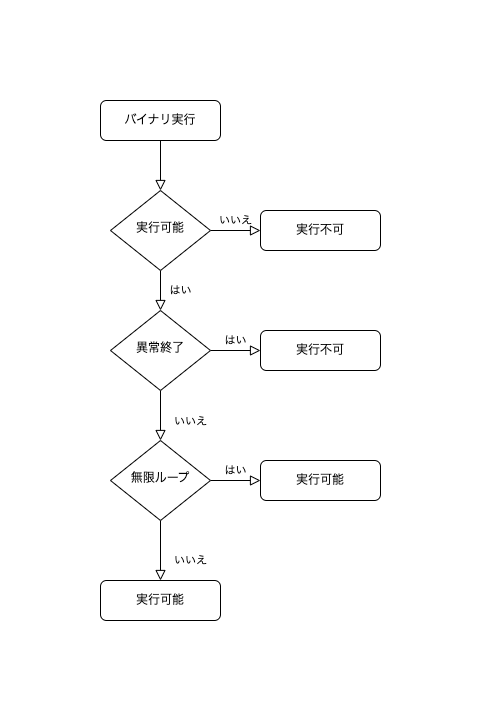
\includegraphics[width=10cm]{img/execflow.png}
		\caption{実行の可否を判定するフローチャート}
		\label{fig:execflow}
	\end{center}
\end{figure}

\subsection{脅威スコア}
本研究では、実行したマルウェアがもたらす脅威の程度を"脅威スコア"として定量化する。尚、本来であればマルウェアの脅威の程度を計測する場合、システムコール呼び出しやパケットの監視などを行い、実際にどのような脅威が発生したかを観測した上で脅威の程度を定量化するのが自然であが、本研究では著者の技術不足のためマルウェアの実際の振る舞いについては観測せず、マルウェアの分類に従った希望的観測による脅威の定量化を行った。

脅威スコアは次のように導出する。まず、"マルウェアの実行の可否"において実行可能であったマルウェアについては、そのマルウェアの分類に応じた相応の脅威が発生したと仮定し、分類に応じた脅威スコアを設定する。マルウェアの分類はインターネット上で提供されているウイルス解析サービスを利用して判定する。分類に応じた脅威スコアを表\ref{tab:typescore}に示す。表\ref{tab:typescore}では、一般に脅威が大きいとされるランサムウェアやバックドアなどは脅威スコアが大きく設定されており、アドウェアやコインマイナーといった比較的脅威が小さいと考えられるものについては脅威スコアが小さく設定されている。表\ref{tab:typescore}を作成するにあたり、セキュリティサービスを提供している企業netscopeが公開しているマルウェアの脅威の分類表\cite{malwareclass}を参考にした。続いて、"マルウェアの実行の可否"において実行不可であったマルウェアについては、そのマルウェアの脅威は発生しなかったと仮定し、脅威スコアは0と判断する。

\begin{table}[htbp]
	\caption{マルウェアの分類と脅威スコアの対応表}
	\label{tab:typescore}
	\centering
	\scalebox{0.64}{
	\begin{tabular}{|c|l|}
        \hline
        脅威スコア & 分類 \\
        \hline
        \hline
        \multirow{8}{*}{3} & Ransomware \\
                & Trojans \\
                & Viruses \\
                & Downloaders \\
                & Backdoors \\
                & Rootkits \\
                & Exploits \\
                & Password Stealers \\
            \hline
            \multirow{1}{*}{2} & Spyware \\
            \hline
            \multirow{8}{*}{1} & Bundlers \\
                & Coinminers \\
                & Adware \\
                & Dialers \\
                & Hoaxes \\
                & Hacktools \\
                & Keygens \\
                & Jokes \\
            \hline
	\end{tabular}
	}\\
\end{table}

\section{環境構築}
\label{環境構築}
ラズビアン環境を用いた評価実験を行うにあたり、実験環境の構築と実行の可否及び脅威スコア導出の自動化を行った。

\subsection{ラズビアン環境の構築}
ラズビアン環境の構築と評価の自動化は図\ref{fig:exparch}のような構成で行った。まず、Ubuntu上でQEMUを動作させRaspberry Pi OSをエミュレートした。QEMUとは、オープンソースのエミュレータ型仮想化ソフトウェアであり、様々なアーキテクチャをエミューレートすることができる。QEMUはマルウェアの動的解析を行う環境として提案されており、動的解析のためのプラグイン\cite{panda}も多く提供されている。本研究では今後、マルウェアの動的解析を行うことを想定してQEMUを採用した。以降、エミュレートしたRaspberry Pi OS環境をゲスト環境と言う。続いて、ゲスト環境にウェブサーバアプリケーションとして、Nginxをインストールした。Nginxは、オープンソースのウェブサーバアプリケーションであり、世界で広く利用されているウェブサーバである。次に、マルウェアのサンプルをゲスト環境に転送することや評価を自動化することを考慮して、ホスト環境からゲスト環境にSSH接続できるようにQEMU及びRaspberry Pi OSの設定を行った。

\begin{figure}[htbp]
	\begin{center}
		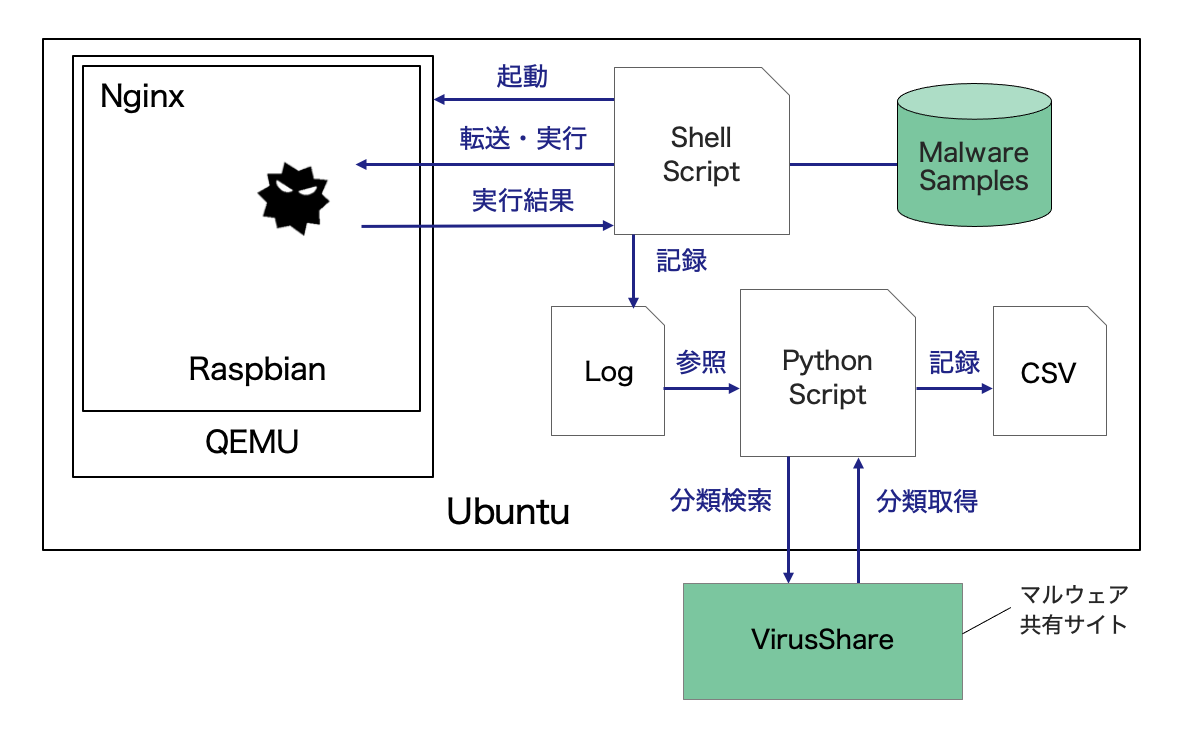
\includegraphics[width=13cm]{img/exparch.png}
		\caption{ラズビアン環境と自動化の構成図}
		\label{fig:exparch}
	\end{center}
\end{figure}

\subsection{評価の自動化}
評価実験では、数百個のサンプルを評価することを想定しており、手動で評価を行うには時間が掛かる。そのため、ゲスト環境の立ち上げ、マルウェアの転送、実行、評価を自動化した。自動化の構成図は図\ref{fig:exparch}の通りである。まず、サンプルごとの実行環境を同じにするため、サンプルごとに新しいゲスト環境を立ち上げる必要がある。ゲスト環境を立ち上げた後、マルウェアをSCPコマンドで転送し、SSHコマンドを用いてマルウェアを実行する。SSHコマンドの終了ステータスからプログラムが正常終了したかどうかなどを判定することができ、終了ステータスが0または124であれば実行可能、終了ステータスがそれ以外であれば実行不可として"マルウェアの実行の可否"を求める。終了ステータス0はプログラムが正常に終了したことを示しており、124はプログラムがタイムアウトしたことを示す。次に、マルウェアの脅威スコアを求める。マルウェアの実行の可否において実行不可と判定されたものについては脅威スコアは0とし、実行可能と判定されたものについては、インターネット上で公開されているマルウェアの検体データベースであるVirusShareでそのマルウェアがどの分類に分類されるかを求め、表\ref{tab:typescore}の分類と脅威スコアの対応表に基づいて脅威スコアを設定する。VirusShareでは、複数のマルウェア解析サービスの解析結果を取得することができる。その解析結果から文字列のパターンマッチングにより最も合致数の多い分類をそのマルウェアの分類とした。最後に、求めた脅威スコアはCSV形式で出力した。
マルウェアの実行の可否を元に脅威スコアを求める工程はPythonプログラムを用い、その他についてはBashShellスクリプトを用いて自動化を行った。


% ============= 評価 =============


\chapter{評価}
\section{実験概要}
本節では、評価実験の概要について述べる。本研究では評価実験として、\ref{環境構築}章で構築したラズビアン環境を用いてマルウェアの実行の可否および脅威スコアを求める実験を行った。本実験の実験環境を表\ref{tab:expenv}に示す。評価に使用するサンプルとして、VirusShareで管理されているマルウェアのうちARMアーキテクチャ上で動作するマルウェアのみをまとめたIoT\_ARMリポジトリ\cite{iotarm}のデータセットを用いた。評価を行う上で、実行可能な形式でないサンプルについては除外した。実験に使用したサンプルの分類内訳を表\ref{tab:sampletype}に示す。

\begin{table}[htbp]
	\caption{実験環境}
	\label{tab:expenv}
	\centering
	\scalebox{0.64}{
	\begin{tabular}{|c|c|c|c|c|}
	\hline
	& OS & CPU & Memory & Architecture\\
	\hline
	Host machine & Ubuntu 22.04.1 LTS(64bit) & Intel Core i7-10750H 2.60GHz*12 & 16GB & x86\_64\\
	\hline
	Sandbox machine & Raspbian Buster 2020.02.14(32bit) & QEMU & 256MB & ARM\\
	\hline
	\end{tabular}
	}\\
\end{table}

\begin{table}[htbp]
	\caption{サンプルの分類内訳}
	\label{tab:sampletype}
	\centering
	\scalebox{0.64}{
	\begin{tabular}{|l|l|}
        \hline
        分類 & サンプル数 \\
        \hline
        \hline
        Trojans & 442 \\
        \hline
        Backdoor & 338 \\
        \hline
        Exploits & 18 \\
        \hline
        Hacktools & 1 \\
        \hline
        Unknown & 2 \\
        \hline
        その他 & 0 \\
        \hline
        \hline
        計 & 801 \\
        \hline
	\end{tabular}
	}\\
\end{table}

また、マルウェアの実行の可否を求める際に無限ループと判定する時間の長さは10秒とした。


\section{実験結果}
801個のサンプルについての脅威スコアの評価結果を表\ref{tab:threatscore}に示す。脅威スコアは合計が1212、平均が1.513、分散が$4.99\times10^-3$という結果が得られた。

\begin{table}[htbp]
	\caption{脅威スコアの結果}
	\label{tab:threatscore}
	\centering
	\scalebox{0.64}{
	\begin{tabular}{|l||l|}
        \hline
        脅威スコア & 1212 \\
        \hline
        平均 & 1.513 \\
        \hline
        分散 & $4.99 \times 10^-3$ \\
        \hline
	\end{tabular}
	}\\
\end{table}

次に、マルウェアの分類別の実行の可否を表\ref{tab:typeresult}に示す。表\ref{tab:typeresult}に示す通り、サンプルのおよそ半数である404個について実行可能となった。分類別に見ると、Trojansは約60\%、Backdoorは約30\%が実行不可という結果となった。また、TrojansとBackdoor以外の分類については全てのサンプルが実行不可となった。

\begin{table}[htbp]
	\caption{マルウェアの分類別の実行の可否}
	\label{tab:typeresult}
	\centering
	\scalebox{0.64}{
	\begin{tabular}{|c||c|c|c|}
        \hline
        & サンプル数 & 実行可能 & 実行不可 \\
        \hline
        \hline
        Trojans & 442 & 176(39.8\%) & 266(60.1\%) \\ % %表示いらない?
        \hline
        Backdoor & 338 & 228(67.4\%) & 110(24.8\%) \\
        \hline
        Exploits & 18 & 0 & 18 \\
        \hline
        Hacktools & 1 & 0 & 1 \\
        \hline
        Unknown & 2 & 0 & 2 \\
        \hline
        その他 & 0 & 0 & 0 \\
        \hline
        \hline
        計 & 801 & 404(50.4\%) & 397(49.6\%) \\
        \hline
	\end{tabular}
	}\\
\end{table}

次に、異常終了時の終了ステータスとその内訳を表\ref{tab:exitstatus}に示す。表\ref{tab:exitstatus}に示す通り、TrojansとBackdoor、Exploitsのいずれにおいても、9割以上が終了ステータス139または127で終了している。終了ステータス139は、プログラムが不正なメモリアドレスを参照した際に出力されるステータスである。終了ステータス127は、不明なコマンドを実行した際に出力されるステータスである。Exploitsに関しては、特に終了ステータス127で異常終了する割合が高く、異常終了したExploitsのサンプルのうち約89\%が終了ステータス127で終了している。

\begin{table}[htbp]
	\caption{異常終了時の終了ステータスとその内訳}
	\label{tab:exitstatus}
	\centering
	\scalebox{0.64}{
	\begin{tabular}{|c|c|c|c|}
        \hline
        Trojans & Backdoor & Exploits & Hacktools \\
        \hline
        \hline
        139(157) & 139(64) & 127(16) & 127(1) \\
        \hline
        127(84) & 127(42) & 139(1) & \\
        \hline
        135(21) & 132(2) & 1(1) & \\
        \hline
        2(3) & 135(1) & & \\
        \hline
        132(1) & 2(1) & & \\
        \hline
	\end{tabular}
	}\\
    \scalebox{0.64}{ 139: 不正なメモリ参照 }
    \scalebox{0.64}{ 127: 不明なコマンドの実行 }
\end{table}

マルウェアの評価時間について、手動で行なった場合はマルウェア1つあたり180秒程度掛かったのに対し、評価の自動化を行なった場合は100秒程度掛かる結果となった。

\section{考察}
本節では、実験結果に対する考察を述べる。

本実験を通して、マルウェア1つあたりに掛かる評価時間が手動の場合に180秒程度掛かっていたところを、評価の自動化により100秒程度まで短縮することが可能であることが示された。このことから、より効率的に評価を行えるという点で、節\ref{環境構築}で提案した自動化手法の有用性が示されたと言えるだろう。

表\ref{tab:threatscore}、および表\ref{tab:typeresult}に示す通り、提案手法により脅威スコアおよび実行の可否を求められることが明らかになった。これら2つの指標によりマルウェアの影響を定量的に示すことができるため、マルウェアの影響を定量的に評価する手法として提案手法の有効性が示されたと言えるだろう。

異常終了時の終了ステータスについて表\ref{tab:typeresult}に示す通り、TrojansとBackdoor、Exploitsのいずれにおいても、9割以上が終了ステータス139または127で終了している。終了ステータス139は不正なメモリアクセスが発生した場合に出力される終了ステータスであり、終了ステータス127は不明なコマンドを実行しようとした際に出力される終了ステータスである。
終了ステータス139が発生した原因として、実行環境がマルウェアの想定している環境と異なっていたことが考えられる。具体的には、OSやカーネルがマルウェアの想定するものとは異なっており、想定していたメモリ管理が行われずメモリアクセス違反が発生したと考えられる。
終了ステータス127が発生した原因としては、マルウェアがプログラム中で使用しているコマンドが実行環境に存在しなかったためであると考えられる。マルウェアの中にはプログラム中で特定のツールのコマンドを呼び出しているものがあるが、そのツールが実行環境に存在しない場合には不明なコマンドの実行となるため終了ステータス127を出力して異常終了することになる。この時、マルウェアが呼び出すコマンドを使用する権限を持っていなかった場合は終了ステータス126を出力して異常終了することになる。
以上のことから、実行環境で利用可能なコマンドを限定する、またはコマンドの実行権限を制限することでマルウェアの脅威を抑制することができると推測される。

% Exploitsが127で終了しているのは特定のツールの脆弱性を狙ったものであるため特定のツールを使用しており、存在しないコマンドの実行によ異常終了が比較的多いと考えられる -> Exploitsを正確に把握できていないので保留


% ============= おわりに =============


\chapter{おわりに}
\section{結論とまとめ}
本研究では、ARMプロセッサのIoT機器を想定した3つの実行環境において、マルウェアが与える影響を定量的に評価する手法を提案し、ラズビアン環境について実際に評価実験を行い、その結果を考察した。本研究の調査から、本研究で提案した評価手法がマルウェアの影響を定量的に評価する手法として有効であることが明らかとなった。また、マルウェアの脅威を抑制するための手段として、利用可能なコマンドを限定する、もしくは権限を制限することが有効であることが示唆された。

\section{今後の課題}
今後の課題として、以下の4点が挙げられる。

\begin{itemize}
	\item 脅威スコアを希望的観測ではなくマルウェアの振る舞いに基づいて算出すること
	\item コンテナ環境及びユニカーネル環境についても評価実験を行うこと
	\item 各環境における影響評価を比較し環境の特性を考察すること
	\item 評価にかかる時間をさらに短縮すること
\end{itemize}

1つ目の課題について述べる。本研究で提案した手法では、脅威スコアをマルウェアの実際の振る舞いではなく分類に基づいて算出した。しかし、この算出方法は希望的観測によるものであり実際の振る舞いを反映していない。より厳密な評価を行うためには、システムコール呼出しや外部との通信、ファイル操作といった実際の振る舞いを解析し、脅威の程度を算出することが必要である。

2つ目の課題について述べる。本研究では評価対象である3つの環境のうちラズビアン環境のみを対象にマルウェアの影響評価を行った。提案手法の有効性を示すためには残り2つの環境についても同様の手法により評価を行い、提案手法がマルウェアの影響を評価する上で有効な手法であることを示す必要がある。

3つ目の課題について述べる。本研究ではラズビアン環境についてのみ影響評価を行いその結果を示したが、各環境の特性を議論するためには残る2つの環境についても評価実験を行いそれらの結果を比較することが必要である。

4つ目の課題について述べる。本研究では、マルウェアの影響評価の手順を自動化することで、手動ではマルウェア1つあたりに180秒程度の評価時間が掛かっていたところを100秒程度まで短縮することを可能にした。しかしながら、数千個以上のマルウェアを評価する場合、数十時間という時間を要するため、提案手法の有用性を向上させるためには更なる時間短縮が望まれる。時間短縮の余地として、QEMUのスナップショット機能を用いることで60秒程度掛かっている実行環境の起動を数秒程度に短縮できると予想している。


% 図\ref{tab:method}に示す.
% \cite{openhab}が挙げられる.

% 図\ref{fig:system}にシステムの全体像を図\ref{fig:system}に示す.
% \begin{figure}[htbp]
% 	\begin{center}
% 		\includegraphics[width=13cm]{assets/sequence.png}
% 		\caption{データがやり取りされるまでのシーケンス図}
% 		\label{fig:sequence}
% 	\end{center}
% \end{figure}


% ==================================

% jbibtex のためのおまじない
\newpage
\bibliographystyle{junsrt}%参考文献の形式
\bibliography{reference}%ここに書く
\renewcommand{\bibname}{参考文献}


\chapter*{謝辞}
本研究を行うにあたり、1年間に渡り多くのご指導をいただいた名古屋大学大学院情報学研究科情報システム学専攻高田広章教授、および名古屋大学大学院情報学研究科情報システム学専攻松原豊准教授に深く感謝いたします。また、日常の議論を通じて多くの知識や示唆をいただいた高田・松原研究室の皆様に深く感謝いたします。特に、元田匡哉氏、坪井正太郎氏には、研究に関して様々な助言をいただきました。深く感謝いたします。


% %
%%%%%%%% 背表紙 (過去のテンプレより拝借)
% 題目を書く.すべて全角で書くべし
\clearpage
\thispagestyle{empty}
\oddsidemargin -2.5in
\evensidemargin -2.5in
\topmargin -.5in
\marginparwidth = 0pt
{
	\tate
	\begin{minipage}{8.0in}
		\small
		%\footnotesize
		\textbf{IoT機器を想定した実行環境におけるマルウェアの影響評価}
		\hfill
		\textbf{2023年2月}
		\hfill
		\textbf{101910020 大羽俊輔}
	\end{minipage}
}
\end{document}